\documentclass{article}
\usepackage{graphicx}
\usepackage[hidelinks]{hyperref}
\hypersetup{colorlinks,urlcolor=blue, linkcolor=black}
\usepackage{url}
\usepackage{amsmath}
\usepackage{float}
\usepackage[numbered]{bookmark}

\begin{document}

\title{D-TACQ LLC system latency measurement guide}
\author{Sean Alsop \\ Contact: \href{mailto:sean.alsop@d-tacq.co.uk}{sean.alsop@d-tacq.co.uk} }

\maketitle

\tableofcontents

\section{Introduction} \label{intro}

\subsection{Overview}
This document serves as a guide to measuring system performance in \mbox{D-TACQ} Low Latency Control (LLC) systems.
Following this guide will allow users to  measure the hardware performance of their LLC system in two distinct modes of operation.
The first mode is a purely hardware mode of operation. This is done using a “zcopy” control program.
This control program is useful for demonstrating the speed of the hardware without any software overhead introduced.
The second mode of operation is performed using the control program known as “cpucopy”.
The cpucopy control program is used to bring some software overhead into the loop – making the latencies involved more representative of a real world control system.
The hardware overhead and software overhead of the LLC system are vital measurements as they set the benchmark for the latencies in the control loop.
\newline
The total system latency is defined as the time between the rising edge of a sample clock and the start of the output of that sample in the analogue output device.
This latency can be directly measured using an oscilloscope, but the latency measurements can also be calculated by the onboard FPGA.
This means that we can have two independent measurements of latency, one measured by the system itself and the other by an independent scope.
If the measurements agree then the user will have a creditable measure of system latency before they start to add on extra control software in the control program.
This report will highlight the steps required to operate the system, view the data on an oscilloscope, measure the self-reported statistics, and will then compare these pieces of information using data acquired at D‑TACQ.
\newline
It is important to note that this report covers only one LLC system configuration, but that other configurations will work with these instructions. The report aims to be as general as is possible. 
\subsection{Representative System}
Our test system used two UUTs, “Local” and “Remote” to simulate a system where AO data is duplicated at a remote location.
\subsection{References}
\begin{enumerate}
	\item \href{http://www.d-tacq.com/resources/d-tacq-4G-acq4xx-UserGuide-r28.pdf}{The \mbox{D-TACQ} 4G User Guide}
	\item \href{http://www.d-tacq.com/resources/LLC_White_Paper.pdf}{The \mbox{D-TACQ} LLC White Paper}
	\item \href{https://github.com/D-TACQ/acq400_hapi}{The \mbox{D-TACQ} acq400\_hapi GitHib repo}
	\item \href{https://github.com/D-TACQ/AFHBA404}{The \mbox{D-TACQ} AFHBA404 GitHib repo}
\end{enumerate}

\subsection{Glossary}
\begin{enumerate}
	\item \textbf{UUT:} Unit Under Test, in this case ACQ2106 with fiber optic comms.
	\item \textbf{HOST:} A Host PC, x86\_64, multi-core.
	\item \textbf{LLC:} Low Latency Control mode, data is transferred one sample at a time.
	\item \textbf{AHFBA404:} Host Bus Adapter, PCIexpress connects UUT and HOST
	\item \textbf{VI:} Vector Input, comprises AI, DI, SPAD : Analog Input, Digital Input, Scratchpad meta-data, pushed from the UUT to the HOST on sample clock.
	\item \textbf{VO:} Vector Output: comprises AO, DO : Analog Output, Digital Output.
	\item \textbf{N mode:} LLC mode with output same cycle
	\item \textbf{N-1 mode:} LLC mode with output next cycle
\end{enumerate}

\subsection{Notation}
\begin{enumerate}
	\item \textbf{command:} indicates name of a program (command)
	\item \verb|preformatted text:| literal input or output from terminal session.
	\item \emph{\textbf{Defined Term:}} some term or acronym specific to this domain (perhaps referenced in the glossary).
\end{enumerate}


\section{Setup and configuration} \label{setup}

\subsection{System overview}
\begin{figure}
	\centering
	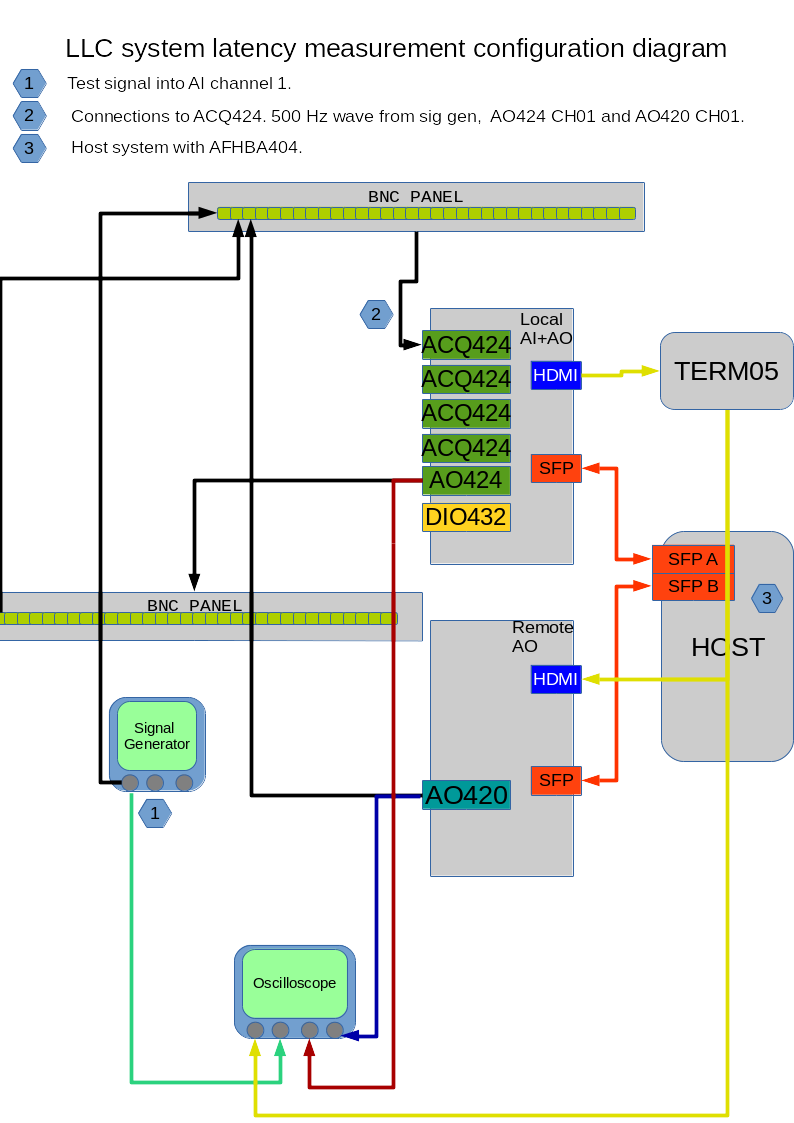
\includegraphics[width=5.0in]{images/remote_ao_diagram_p.png}
	\caption{The system connections.}
	\label{systemconnections}
\end{figure}

\subsection{Firmware \& software versions on the acq2106 systems}
The systems used in this document are set up as follows: 
\newline
\textbf{acq2106\_085:} 4*acq424 + ao424 + dio432
\newline
\textbf{acq2106\_153:} ao420 (in site 5)
\newline
For full firmware version info, see Appendix C: Firmware Versions
\subsection{Turnkey Clock Setup}
The master system (acq2106\_085) takes a front panel clock and divides it down to either 20kHz or 50kHz (using sync\_role to change the clock speed).
It then feeds this clock out to the slave system (acq2106\_153) and the oscilloscope.
This configuration can be seen in detail from the rc.user files on each board which are included below.

\begin{verbatim}
acq2106_085> cat /mnt/local/rc.user
# DEFAULT init for acq425, 1000000 Hz, auto soft trigger
/usr/local/epics/scripts/wait_ioc_ready
/usr/local/CARE/acq2106\+acq42x.init
# Local clock and soft trigger
# Alternate front panel clock and front panel trigger
set.site 0 sync_role fpmaster 20000 1000000
# For other combinations try 'set.site 0 sync_role help'
# Customisation for LLC:
set.site 1 trg 1,1,1
set.site 5 clk 1,2,1
set.site 5 clkdiv 1


acq2106_153> cat /mnt/local/rc.user
# DEFAULT init for acq424, 1000000 Hz, auto soft trigger
/usr/local/CARE/acq2106\+acq42x.init
# Local clock and soft trigger
set.site 0 sync_role slave
# Alternate front panel clock and front panel trigger
#set.site 0 sync_role fpmaster 1000000 1000000
# For other combinations try 'set.site 0 sync_role help'
# Added customisation for LLC here.
set.site 5 clk 1,1,1
set.site 5 trg 1,1,1
set.site 5 dac_range_ALL 1
set.site 5 clkdiv 1
soft_trigger
\end{verbatim}

\section{Enable Latency Instrumentation in FPGA} \label{latency_intrumentation}
There are a number of FPGA registers that can be used to analyse the latency of the LLC system.
There registers can be used to calculate several statistics on the performance of the system.
The registers can be accessed from an ssh session on the acq2106 and are located in the DAC site (which is site 5 in the specified configuration).
The recommended usage, however, is to encode the registers latency information into the data scratch pad.
To do this run the following command in an ssh session:

\begin{verbatim}/usr/local/CARE/LLC_instrument_latency\end{verbatim}

\section{Setting up the host computer} \label{settinguphost}
The recommended host OS is the latest flavour of CentOS 7 Linux (7.6 or better).

\begin{verbatim}
cat /etc/redhat-release 
CentOS Linux release 7.6.1810 (Core) 
uname -a
Linux seil 3.10.0-957.21.3.el7.x86_64 #1 SMP Tue Jun 18 16:35:19 UTC 2019
x86_64 x86_64 x86_64 GNU/Linux
\end{verbatim}

Once the AFHBA404 has been inserted into a CPU PCIe slot (make sure not to choose a PCH PCIe slot as this greatly impacts latency), boot the computer and clone the driver from:
\newline
\href{https://github.com/D-TACQ/AFHBA404}{https://github.com/D‑TACQ/AFHBA404}
\newline
For ease of use \mbox{D-TACQ}  recommends cloning the above git repository to the following directory:

\begin{verbatim}
/home/$USER/PROJECTS/AFHBA404
\end{verbatim}

Once the repository has been cloned, open a terminal in the newly cloned directory and enter the command:

\begin{verbatim}
make
\end{verbatim}

Once make has compiled all of the code the user can load the driver by running the following command:

\begin{verbatim}
sudo ./scripts/loadNIRQ
\end{verbatim}

Once the driver has been successfully loaded connect fibre cables to the AFHBA404 in the host computer and connect the other end to the acq2106 systems.
Once the connections have been made and the acq2106 booted the following script can be used on the host to verify that the connection has been established via the fibre cable:

\begin{verbatim}
./scripts/get-ident-all
\end{verbatim}

This should list all of the acq2106 systems attached to the host computer. In our system we see:

\begin{verbatim}
[dt100@seil AFHBA404]$ sudo ./scripts/get-ident-all 
seil 0 acq2106_085 A
seil 1 acq2106_153 A
\end{verbatim}

This translates as:
\begin{verbatim}
Host 'seil' DEVNUM=0 (AFHBA404 A), acq2106_085 ('Local UUT'), Comms A
Host 'seil' DEVNUM=1 (AFHBA404 A), acq2106_153 ('Remote UUT'), Comms A
\end{verbatim}

If the systems connected are not listed then please consult the driver documentation found in the git repository found in the link above.

\section{Configuring the ACQ2106 UUTs}\label{configure2106s}
Once the acq2106 systems have been connected to the host computer they can be configured for LLC operation by using a python script found in the git repo cloned in the last step.
The script is found in the scripts/ directory.
It should be used as follows:
\begin{verbatim}
python ./llc-config-utility.py [1st UUT name] [2nd UUT name]
\end{verbatim}

so in our example:

\begin{verbatim}
python ./llc-config-utility.py acq2106_085 acq2106_153
\end{verbatim}

\section{Host-Side Control Programs} \label{controlprogs}

\subsection{zcopy}

The \textbf{zcopy} program sets the \textbf{VO} source buffer to be the same address as the \textbf{VI} target buffer.
This means that the outputs are updated from the inputs without any host-side CPU intervention.
While this is of course not representative of a real control system, it does demonstrate the performance of the hardware.

\subsection{cpucopy}
The cpucopy program sets separate VI target and VO source buffers, and relies on using the HOST CPU to copy data from target to source.
This is more representative of a control system, but requires addition real time setup and interpretation.
\subsection{Procedure}
There are four control programs available for use.
\mbox{D-TACQ} recommends starting with the zcopy control programs before moving to the cpucopy control programs.
There are two versions of each zcopy and cpucopy – one for a single box use case, and another for two systems.
This guide will be demonstrating the two box case, but if the user only has one system then use the single box control programs.
There is some user input required during this step if the control programs have not been run before.
However, these commands are usually provided in a factory acceptance test provided at delivery with the LLC system.
Shell variables reference the control program path and number of samples (1M):
\begin{verbatim}
LLC=/home/dt100/PROJECTS/AFHBA404/LLCONTROL/
NSAM=1000000
\end{verbatim}

\subsubsection{Two-Box Operation}
The \textbf{zcopy} command for the two box system evaluated in this report is as follows:

\begin{verbatim}
sudo VERBOSE=1 NCHAN=128 AOCHAN=32 DO32=1 SPADLONGS=16 \
LLC/afhba-llcontrol-zcopy-remote-ao $NSAM
\end{verbatim}

The \textbf{cpucopy} command for the two box system is:
\begin{verbatim}
sudo DUP1=96 VERBOSE=1 NCHAN=128 AOCHAN=32 DO32=1 SPADLONGS=16 \
LLC/afhba-llcontrol-cpucopy-AIAO-AO $NSAM
\end{verbatim}

\subsubsection{Single-Box Operation}

Using the “local UUT” only, the zcopy command would be:
\begin{verbatim}
sudo VERBOSE=1 NCHAN=128 AOCHAN=32 DO32=1 SPADLONG S=16 \
LLC/afhba-llcontrol-zcopy $NSAM
\end{verbatim}

and the cpucopy command would be:

\begin{verbatim}
sudo DUP1=96 VERBOSE=1 NCHAN=128 AOCHAN=32 DO32=1 SPADLONGS=16 \
LLC/afhba-llcontrol-cpucopy $NSAM
\end{verbatim}

\section{Modes of operation} \label{modes}

There are two different delay types (which are covered in far more depth in \href{http://www.d-tacq.com/resources/LLC_White_Paper.pdf}{the \mbox{D-TACQ} LLC White Paper}).
These modes are \textit{\textbf{N}} and \textit{\textbf{N-1}}.
Which mode is used depends on the circumstances and requirements and in this guide both modes are shown.
In order to configure a system for the best possible latency measurement \textit{\textbf{N mode}} is used. To change between \textit{\textbf{N and N-1 modes}} an OUTPUT\_DELAY parameter is set on the acq2106.
To configure zcopy for \textit{\textbf{N mode}} the OUTPUT\_DELAY should be set during an ssh session prior to starting the shot.
It should be set to approximately 1.9 $\mu$s as shown below.

\begin{verbatim}
set.site 5 OUTPUT\_DELAY 1.9
\end{verbatim}

Note that the same OUTPUT\_DELAY will not work for cpucopy applications as there is a software overhead.
For cpucopy an OUTPUT\_DELAY of 4.36 was used (shown later in the guide).
The OUTPUT\_DELAY used for each specific users case should be approximated, and then tested.

Note also, that this value allows no time for the HOST CPU algorithm see section \ref{nmodepcs}.

\section{Starting the LLC capture on acq2106} \label{startingcap}
Once the control program has been started the capture can begin by either transient capture or continuous (streaming) capture.
This document will cover the streaming data case.
In order to start a stream, the user can connect to port 4210 using nc(1) as shown:

\begin{verbatim}
nc acq2106_085 4210 > /dev/null
\end{verbatim}

The user can also use pv(1) to view the data rate as it moves through the pipe:

\begin{verbatim}
nc acq2106_085 4210 | pv > /dev/null
\end{verbatim}

The data streamed from the port is directed to /dev/null as a copy is always stored by the control program (both cpucopy and zcopy).
Once the stream has started data will start to appear on the host in the directory from which the control program was run.
Once the number of samples has been reached and the control program stops the stream should be stopped by the user.

\section{Analysing the results} \label{analysis}
\subsection{zcopy results}
The data acquired on the host computer can be analysed using the following python script:

\begin{verbatim}
python ./llc_spad_reg_histogram.py acq2106_085
\end{verbatim}

This script will read the data sitting in the AFHBA404 directory on the host and plot histograms of the data encoded in the spad by the acq2106.
The following graphs were obtained using the method explained above:

The histograms were sampled at 1kHz, so for a sample rate 20kHz we have one histogram point per 20 ADC samples, and at a sample rate 50kHz we have one histogram point per 50 ADC samples.
The FPGA takes the maximum of the last 64 samples, so no samples are missed. See section \ref{spadregmap} for detail on the registers available. Note that the histogram points are maximum latency per period, so we do not miss any extreme outliers by averaging latencies.

\subsubsection{zcopy at 20kHz}

\begin{figure} [htb!]
	\centering
	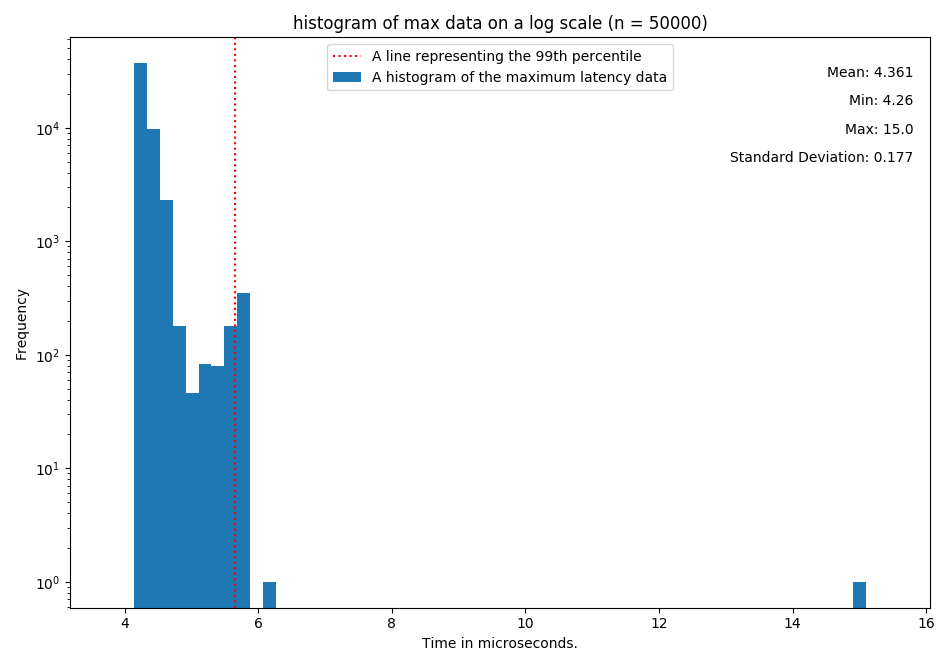
\includegraphics[width=4.0in]{images/better_images/20kHz_final_small.png}
	\caption{Histogram of maximum latency in zcopy mode. Clock rate 20kHz. Intel core i7 CPU.}
	\label{zcopy20hist}
\end{figure}


\begin{figure} [htb!]
	\centering
	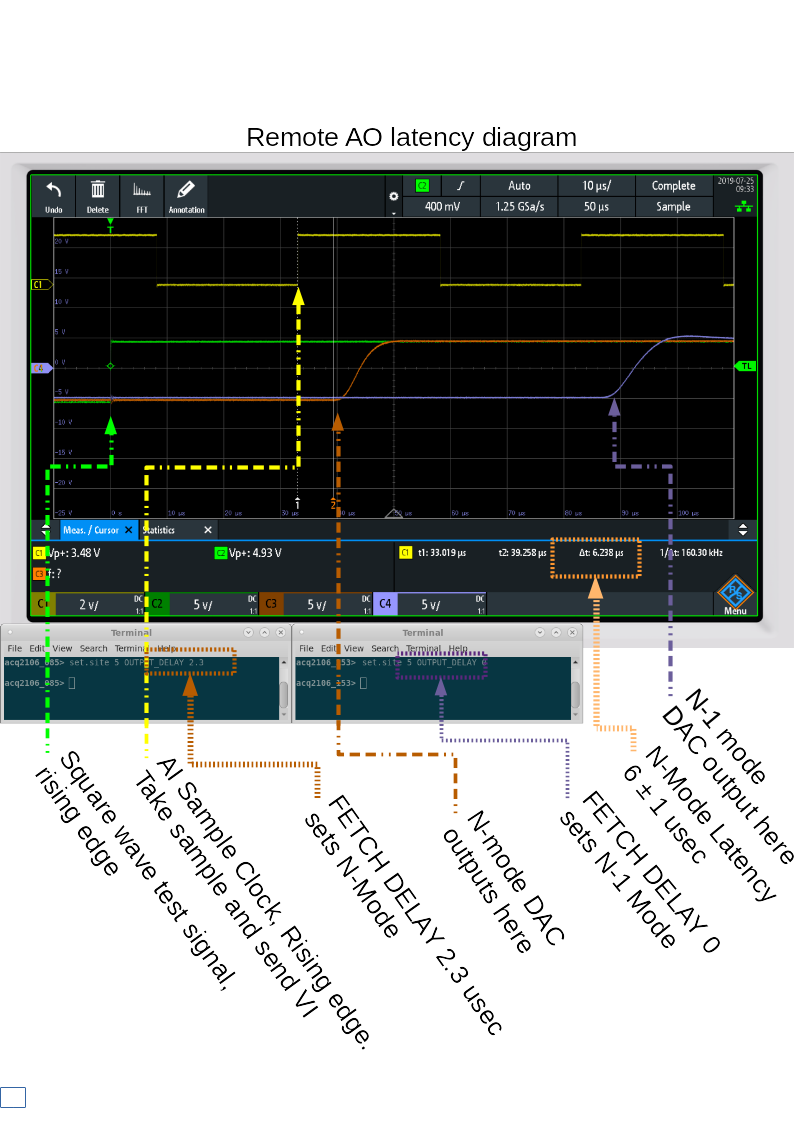
\includegraphics[width=4.0in]{images/20kHz_annotated_scope-p-2.png}
	\caption{A scope trace taken of two systems in zcopy mode “Local”, “Remote” at 20kHz.}
	\label{zcopy20scope}
\end{figure}

From figures \ref{zcopy20hist} and \ref{zcopy20scope} it can be seen that the performance of the system in zcopy mode at 20kHz (hence zero software overhead) is very uniform.
The average latency is 4.3$\mu$s.
There is a single outlier sample at 15$\mu$s which means that access to RAM must have been blocked for 15$\mu$s.
Since this was observed during a zcopy run this is not a timeslice effect.

Figure \ref{zcopy20scope} shows end-to-end latency of approximately 6$\mu$s $\pm$ 1$\mu$s in N mode.
Figure \ref{zcopy20scope} also illustrates the difference between N mode and N-1 mode (where adding the correct delay to the fetch results in improved latency).
The terminal windows show how the OUTPUT\_DELAY is set and the result is observed as the rising edge appearing earlier in N mode.

\subsubsection{zcopy at 50kHz}

\begin{figure} [htb!]
	\centering
	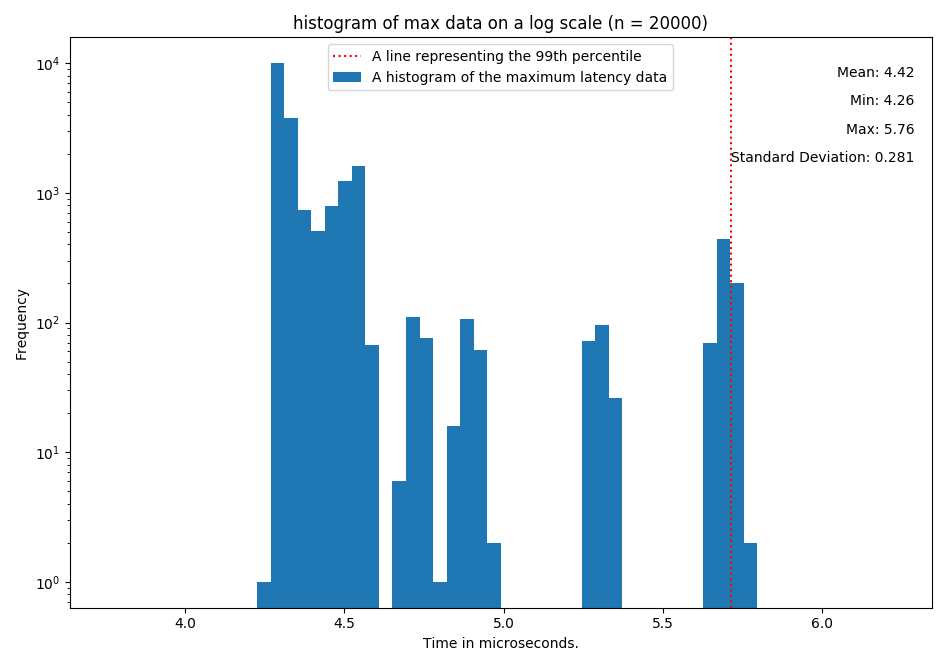
\includegraphics[width=4.0in]{images/better_images/50kHz_final_small.png}
	\caption{Histogram of maximum latency in zcopy mode. Clock rate 50kHz. Intel core i7 CPU.}
	\label{zcopy50hist}
\end{figure}

\begin{figure} [htb!]
	\centering
	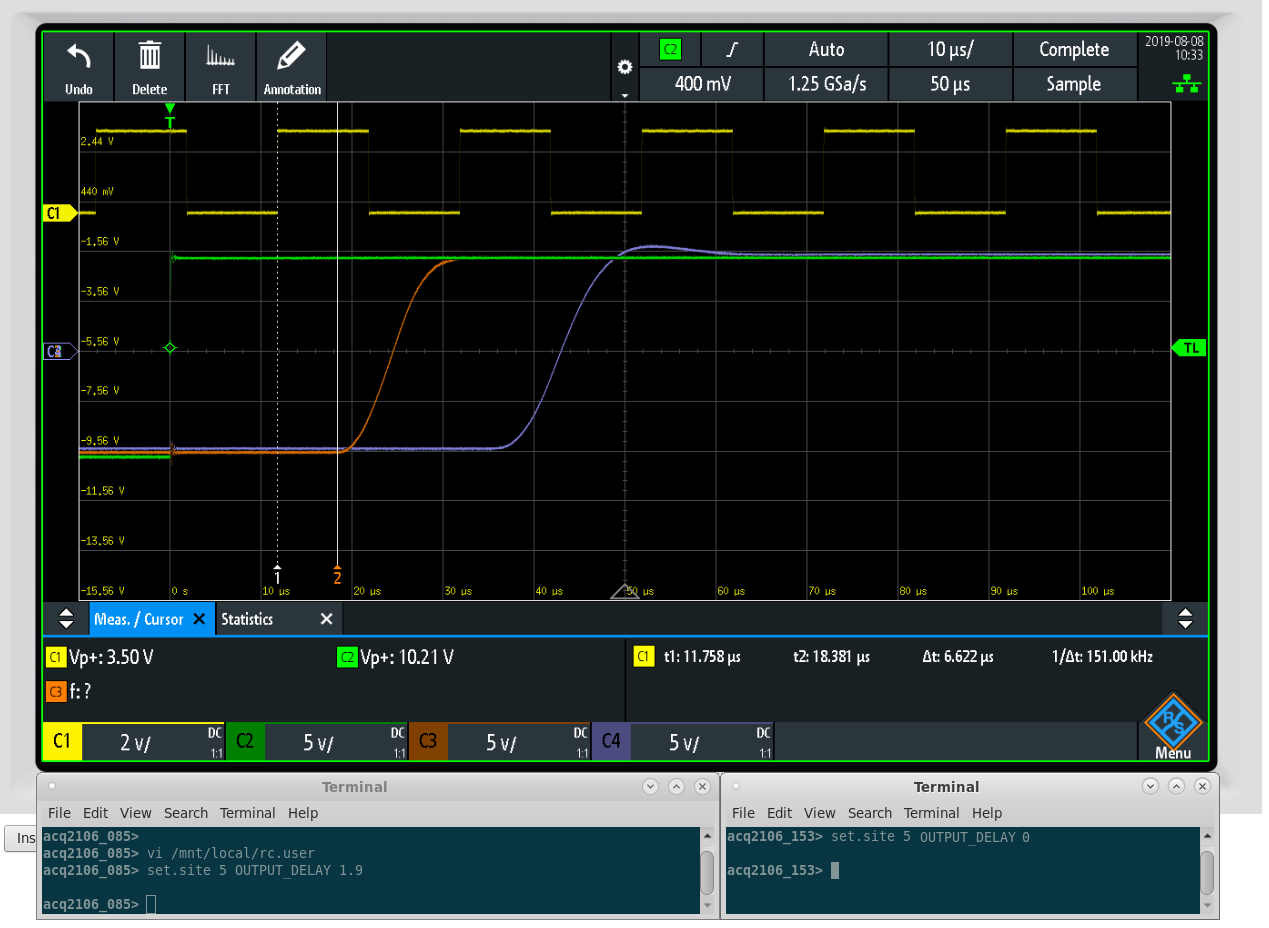
\includegraphics[width=4.0in]{images/50kHz_annotated_scope_2.png}
	\caption{A scope trace of two systems at 50kHz (zcopy mode) showing an approximate overall latency of 7 $\mu$s $\pm$ 1$\mu$s.}
	\label{zcopy50scope}
\end{figure}

Figures \ref{zcopy50hist} and \ref{zcopy50scope} demonstrate a similar latency result to the system operating at 20kHz.
Comparing the packet latencies in figures \ref{zcopy20hist} and \ref{zcopy50hist} to the total system latencies of the scope gives some indication of the times involved in the control path.
From the rising clock edge of the sample clock, to the host, and back to the acq2106 takes approximately 4.4$\mu$s.
From the scope trace and the knowledge of OUTPUT\_DELAY we can also determine that the time from rising sample clock edge to that same data packet arriving on the host is 1.9$\mu$s.
This is verified by the second system appearing much later in the scope trace (the request for data arrives before the data does on the host).
The stated latency of 1.9$\mu$s is not calculable due to the nature of the zcopy operation. Values are explained in more depth in the \mbox{D-TACQ}  LLC White Paper. \\
If we perform the following calculation:
\begin{equation}
\text{Time measured on scope} - \text{Time measured by FPGA} = \text{Time for DAC to output}
\end{equation}
This leaves approximately 2 $\mu$s ($6-4$  $\mu$s, as in the equation above) for the DAC to output the packet it receives from the host.

\newpage

\subsection{cpucopy results}
A similar process can be undertaken to analyse the data from a cpucopy run at 20kHz and 50kHz.
The same python script can be used to plot the histograms automatically:

\begin{verbatim}
python ./llc_spad_reg_histogram.py acq2106_085
\end{verbatim}

\subsubsection{cpucopy at 20kHz}

\begin{figure} [htb!]
	\centering
	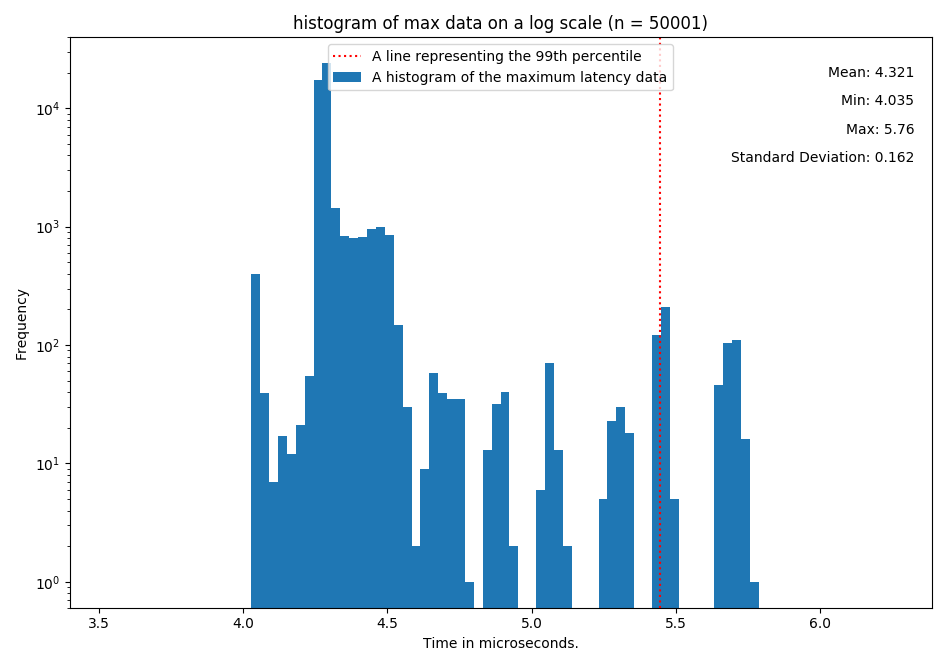
\includegraphics[width=4.0in]{images/better_images/20k_cpu.png}
	\caption{A histogram of the FPGA maximum register during a cpucopy run at 20kHz}
	\label{cpu20hist}
\end{figure}

\begin{figure} [htb!]
	\centering
	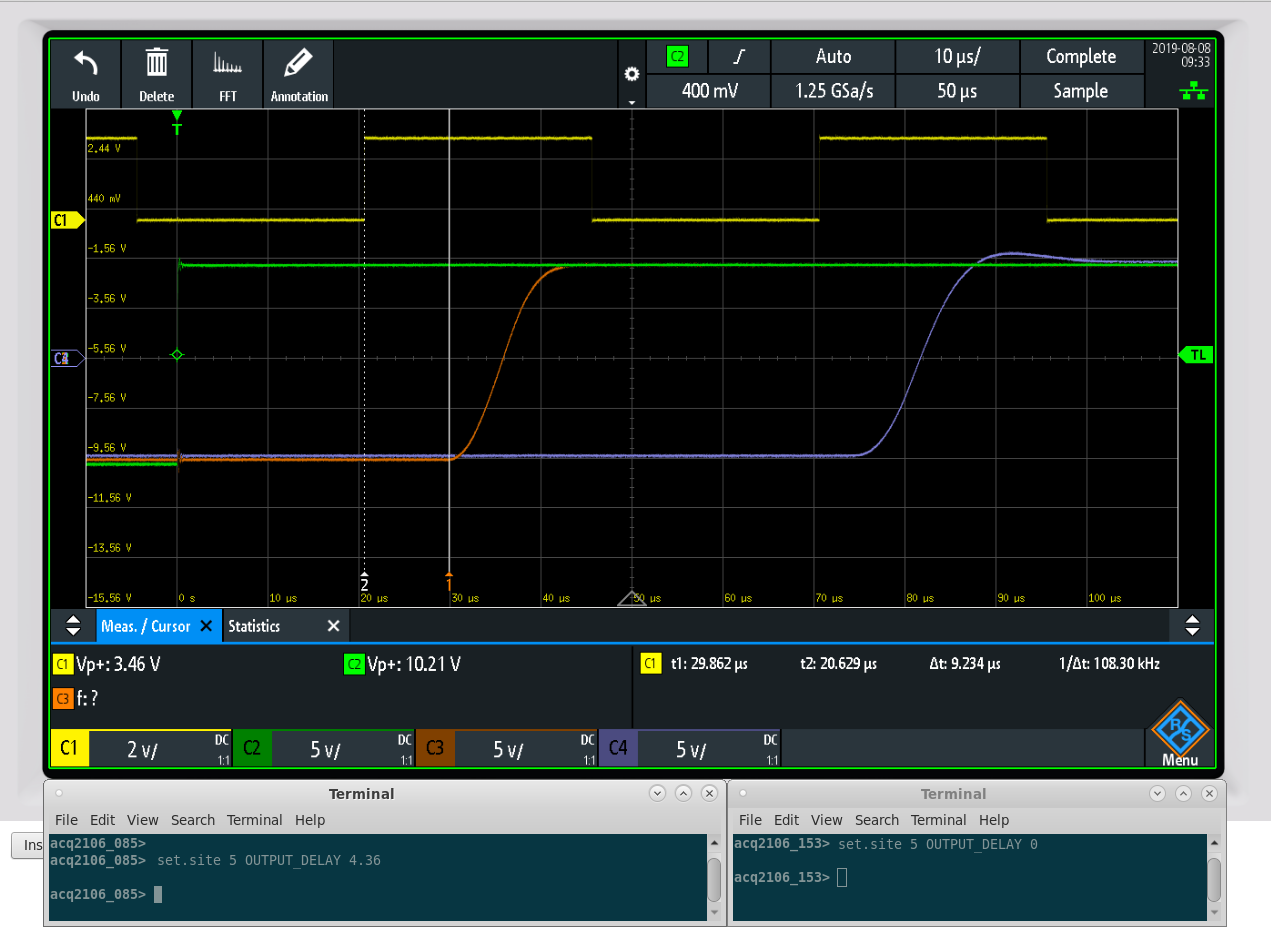
\includegraphics[width=4.0in]{images/20kHz_annotated_scope_cpucopy_2.png}
	\caption{A scope trace of a cpucopy run at 20kHz. Latency is approximately 9 $\mu$s $\pm$ 1$\mu$s.}
	\label{cpu20scope}
\end{figure}

The 20kHz cpucopy histogram (figure \ref{cpu20hist}) looks similar to the zcopy histogram (figure \ref{zcopy20hist}) because the FPGA registers are measuring hardware latency.
This is the latency for the previous packet.

\subsubsection{cpucopy at 50kHz}

\begin{figure} [htb!]
	\centering
	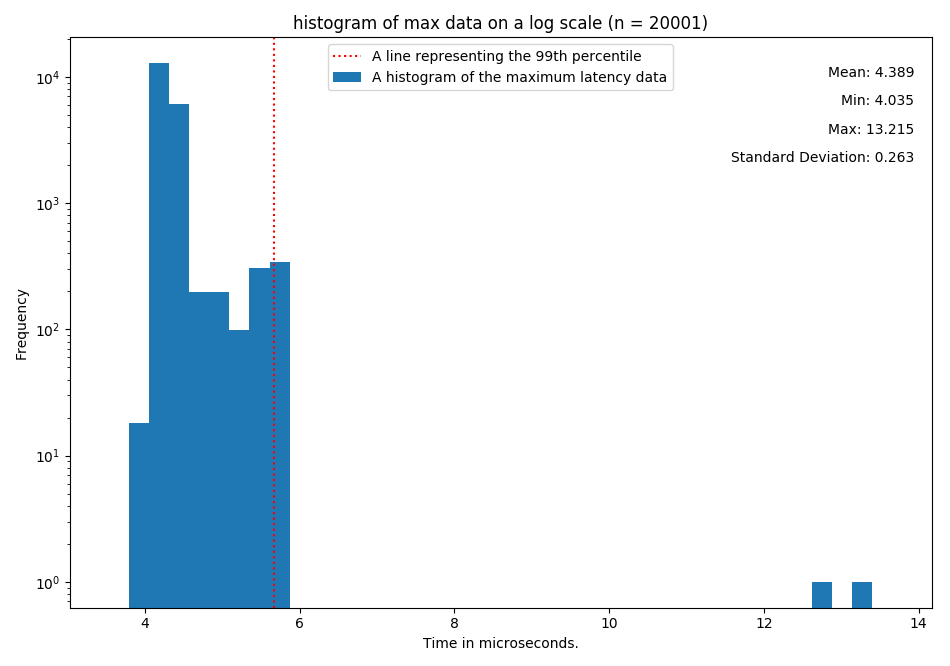
\includegraphics[width=4.0in]{images/better_images/50kHz_cpu.png}
	\caption{A histogram of the FPGA maximum register during a cpucopy run at 50kHz}
	\label{cpu50hist}
\end{figure}

\begin{figure} [htb!]
	\centering
	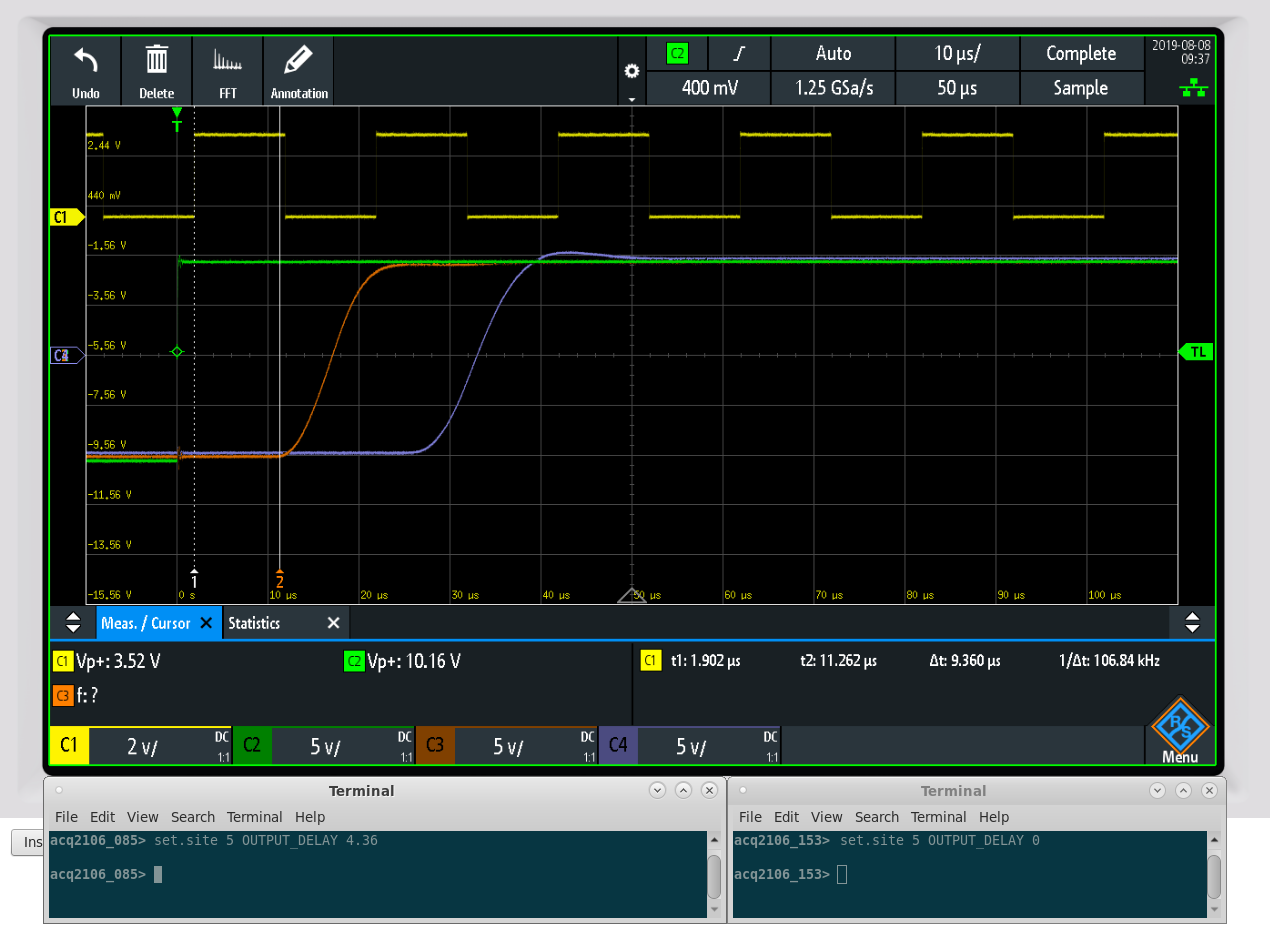
\includegraphics[width=4.0in]{images/50kHz_annotated_scope_cpucopy_2.png}
	\caption{A scope trace of a cpucopy run at 50kHz. Latency is approximately  9 $\mu$s $\pm$ 1$\mu$s.}
	\label{cpu50scope}
\end{figure}

The results for cpucopy at 50kHz are fairly similar to those observed at 20kHz.
In figure \ref{cpu50hist} there are two samples out at the far right of the histogram past 12$\mu$s.
This is another example of the CPU missing the sample and not sending the most up to date sample to the AO until the next PCIe request is received.
It is more illustrative to look at the scope traces for a cpucopy run.
The scope traces show that the latency is increased by approximately between 2 and 3$\mu$s when operating in the cpucopy mode rather than in zcopy mode.
This is directly demonstrating the effect of forcing the software to copy the AI data to the AO buffer, as there is very little time spent doing anything else in a cpucopy control loop.
This is explored in more detail in the next section.

\newpage
\subsection{Discussion}
Note that clock speed does not affect hardware latency as detailed in figures \ref{cpu20hist} and \ref{cpu50hist}.
What does affect the final latency is the time the CPU has to perform a calculation on the data it has before it is available to the analogue outputs.
A faster clock means that the CPU has less time to perform a calculation as the next sample will be incoming.
This is an important concept as it is up to the user to write the control, and hence set the appropriate OUTPUT\_DELAY.
The OUTPUT\_DELAY determines whether the system is operating in \textit{\textbf{N or N-1 mode}}.
The difference in OUTPUT\_DELAY values between cpucopy and zcopy modes is attributed to the time for the CPU to fetch the sample values from RAM.
This can be estimated from the difference in time between the zcopy OUTPUT\_DELAY and the cpucopy OUTPUT\_DELAY.

So the RAM access time calculation should be:

\begin{equation*}
	\text{(cpucopy OUTPUT\_DELAY)} - \text{(FULL zcopy OUTPUT\_DELAY)}
\end{equation*}

or:

\begin{equation*}
	4.36 - 1.886 = 2.474 \mu s
\end{equation*}

Compared to Scope:

\begin{equation*}
\text{(cpucopy scope latency at 20kHz)} - \text{(zcopy scope latency at 20kHz)}
\end{equation*}

or:

\begin{equation*}
	9\pm 1 - 6\pm 1 = 3\pm 2 \mu s \text{ (20kHz)}
\end{equation*}

\begin{equation*}
\text{(cpucopy scope latency at 50kHz)} - \text{(zcopy scope latency at 50kHz)}
\end{equation*}

or:

\begin{equation*}
9\pm 1 - 6\pm 1 = 3\pm 2 \mu s \text{ (50kHz)}
\end{equation*}

This is including the error reading the scope (instrument resolution error).
The RAM access time is an important value to understand, as this needs to be performed every iteration of the control loop in order to check that all the data has arrived.
\subsection{Calculated vs observed latencies}

\begin{center}
	\begin{tabular}{||c c c||} 
		\hline
		Mode and frequency & \multicolumn{1}{|p{3cm}|}{\centering Reported register values \\+ OUTPUT\_DELAY ($\mu$s)}
		 & \multicolumn{1}{|p{3cm}|}{\centering Latency observed\\on scope ($\mu$s)} \\ [0.5ex] 
		\hline\hline

		\hline
		zcopy (20kHz) & 4.3 + 1.9 = \textbf{6.2} & \textbf{6 $\pm$ 1}\\
		\hline
		zcopy (50kHz) & 4.3 + 1.9 = \textbf{6.2} & \textbf{7 $\pm$ 1}\\
		\hline
		cpucopy (20kHz) & 4.1 + 4.4 = \textbf{8.5} & \textbf{9 $\pm$ 1}\\
		\hline
		cpucopy (50kHz) & 4.1 + 4.4 = \textbf{8.5} & \textbf{9 $\pm$ 1}\\ [1ex]
		\hline
	\end{tabular}
\end{center}

As can be seen from the tables above the observed latencies are very close to the latencies reported by the registers.
The uncertainties in the scope measurement have been taken as half of the smallest division ($\pm 1 \mu s$) and so the FPGA measurements are well within margin of error for the observed scope latencies.

\section{Conclusion} \label{conc}
In conclusion there are two reliable methods of measuring latency.
One method relies on hardware registers to report the hardware latency of the system and the second relies on an oscilloscope independent of the control system.
These values, when compared, allow insight into how the system works.
We present a method of automated in-system latency measurement that matches external timing measurement, so it can be used with confidence both for hardware characterisation using zero copy, and for tuning user algorithms with real calculations in \textit{\textbf{N-mode}}.

\newpage

\section{Appendix A: LLC on an Intel Xeon} \label{xeon}

\begin{figure}[!htb]
	\centering
	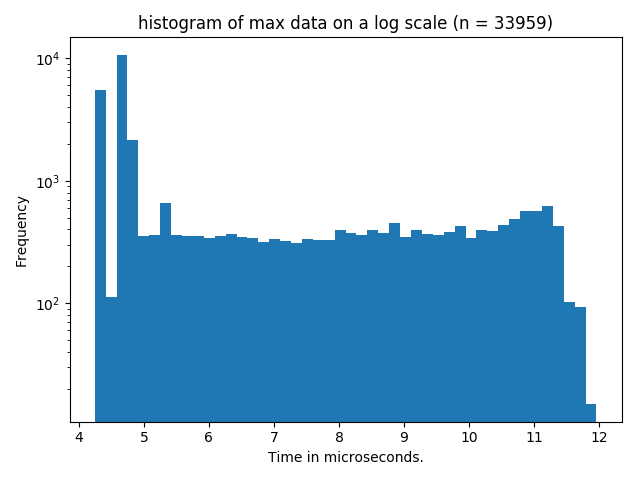
\includegraphics[width=4.0in]{images/50kHz_xeon.png}
	\caption{Histogram of maximum latency. Clock rate 50kHz. Intel Xeon CPU.}
	\label{xeon50}
\end{figure}

Figure \ref{xeon50} is the test from figure \ref{zcopy50hist} repeated on a XEON (multi-processor) system.
We see that the maximum latency doubles to 12$\mu$s, but more significantly, the number of “slow cycles” is greatly increased.
We suspect that this is due to a more complex memory architecture on the multiprocessor system (ECC and/or memory shared between multiple processor sockets).
XEON systems are traditionally preferred for big PCS systems to maximise the number of compute cores, however, for very high clock rates, a desktop class CPU may give better results.
This is possibly a good application for \mbox{D-TACQ} “Alternate Target” technology - send the most time-critical data to one box with a simple algorithm running on a uni-processor, send less time-critical data on a slower schedule to the multi-processor box.

\newpage

\section{Appendix B: Example "N-Mode PCS"} \label{nmodepcs}

Setting OUTPUT\_DELAY to the minimum required to achieve \textit{\textbf{N-Mode}} shows the performance of the hardware but leaves no time for any practical control algorithm in the HOST CPU.



Fig \ref{20repscope} shows a system is programmed with a OUTPUT\_DELAY of 10$\mu$s at 20kHz.
This gives the CPU approximately (10-4.5 = 5.5) $\mu$s to perform the required control algorithm.
This assumes a very fast output calculation!.
Note that OUTPUT\_DELAY could be increased to 20, 30 $\mu$s, allowing 15, 25$\mu$s for calculation and still improve on \textit{\textbf{N-1 Mode}}.

\begin{figure} [htb!]
	\centering
	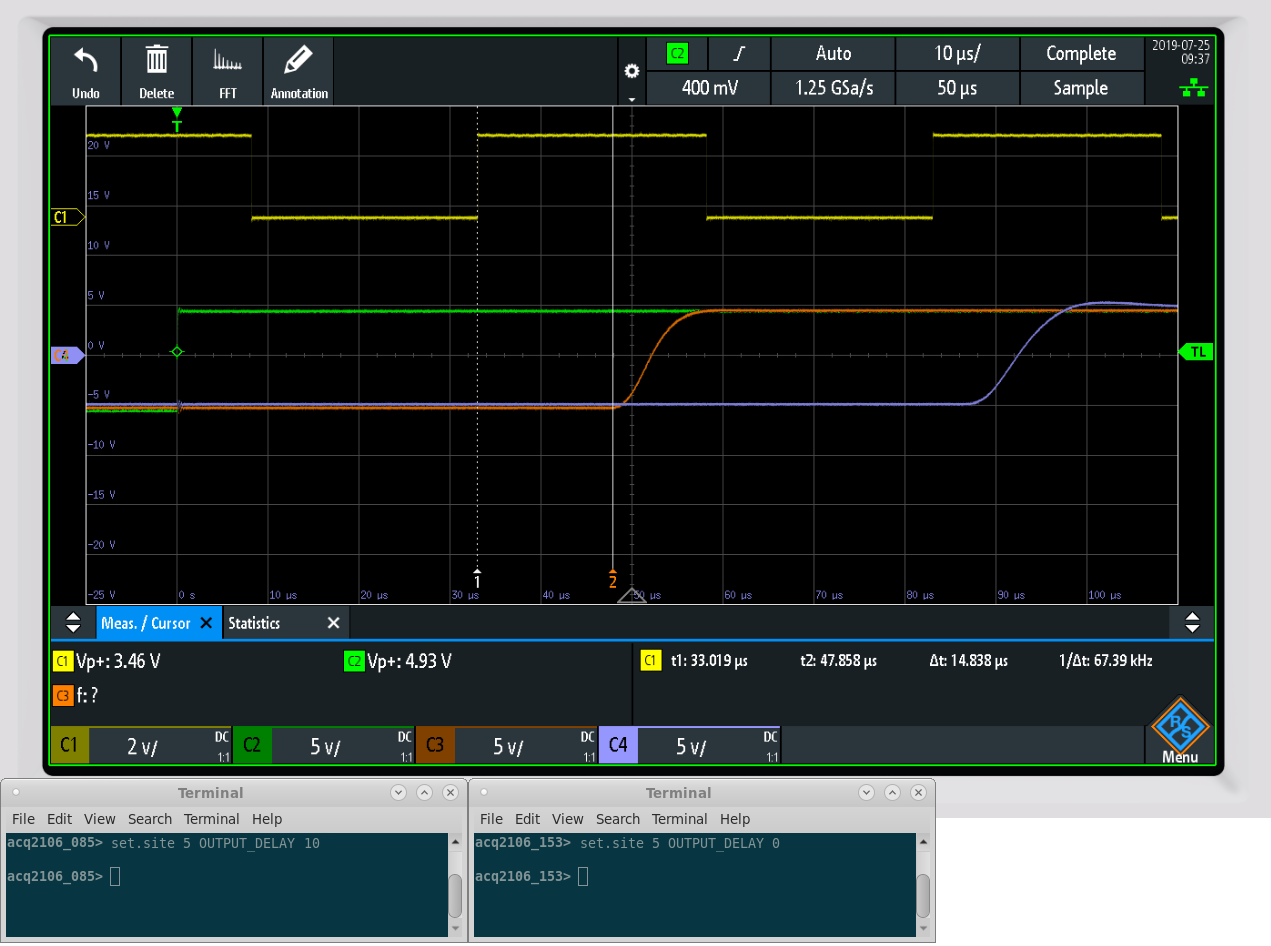
\includegraphics[width=4.0in]{images/n-mode-pcs-scope-trace-20kHz-2.png}
	\caption{An example PCS system with a more representative OUTPUT\_DELAY of 10$\mu$s at 20kHz.}
	\label{20repscope}
\end{figure}

\begin{figure} [htb!]
	\centering
	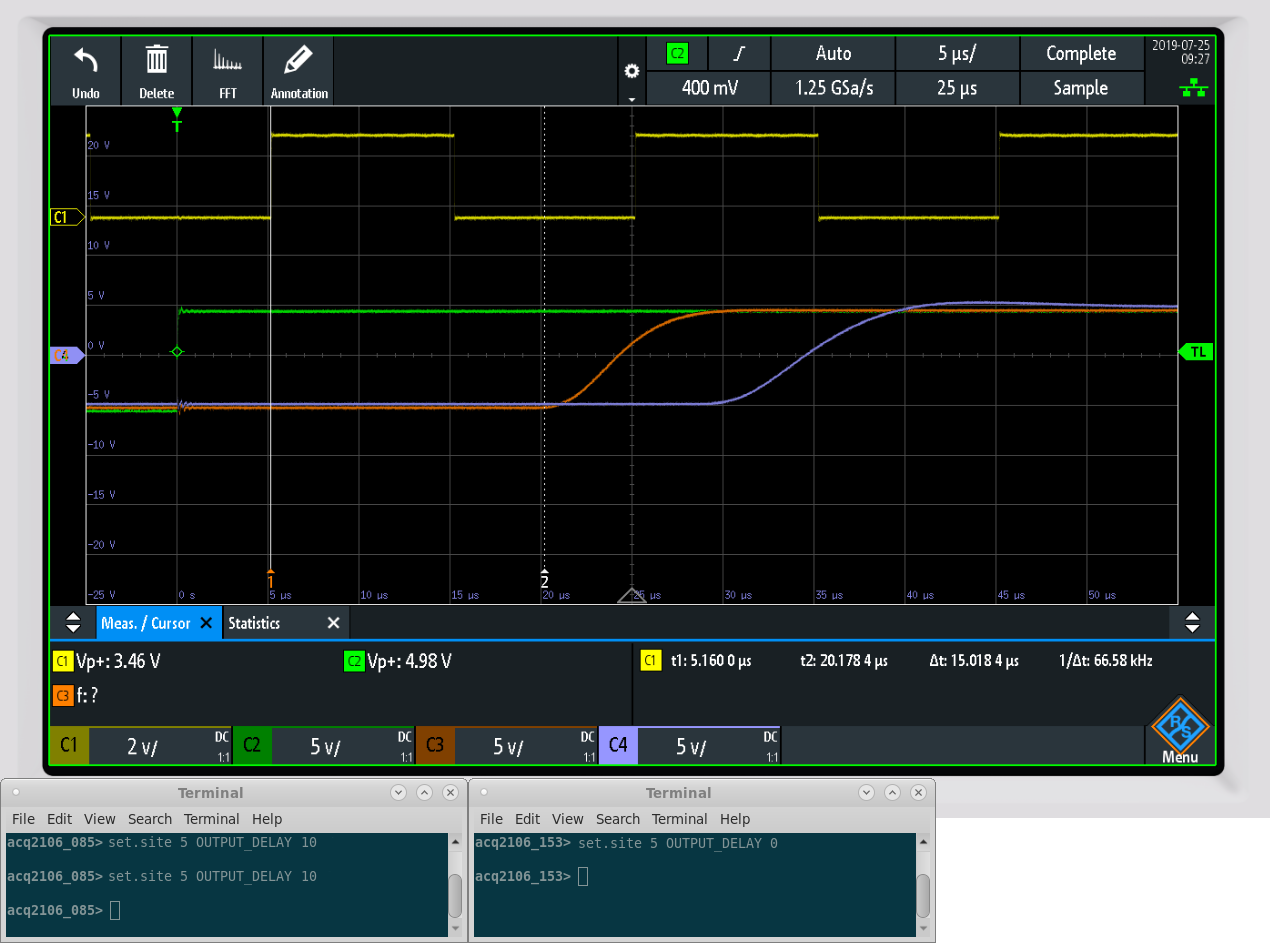
\includegraphics[width=4.0in]{images/n-mode-pcs-scope-trace-50kHz-2.png}
	\caption{An example PCS system with a more representative OUTPUT\_DELAY of 10$\mu$s at 50kHz.}
	\label{50repscope}
\end{figure}

Figure \ref{50repscope} is a scope trace with the same OUTPUT\_DELAY, 5$\mu$sec processing, but now at 50kHz.
Note that the improvement in latency over the \textit{\textbf{N-1 Mode}} is reduced.
We suggest this means that for 50kHz and above, \textit{\textbf{N-1 Mode}} is best.
\textit{\textbf{N Mode}} will give increasingly better results as the clock rate is reduced.

\newpage

\section{Appendix C: SPAD register map} \label{spadregmap}

\begin{center}
	\begin{tabular}{||c c c||} 
		\hline
		Register & Agent & Description \\ \hline\hline\hline
		0 & FPGA & Sample Count \\
		\hline
		1 & FPGA & $\mu$s \\
		\hline
		2 & HOST & pollcat : busy wait time $>$1 is good \\
		\hline
		3 & HOST & difftime\_$\mu$s abs wait for sample \\ [1ex] 
		\hline
		4 & FPGA/A9 Timer & Latency : LATEST | AVERAGE \\
		\hline
		5 & FPGA/A9 Timer & Latency : MIN | MAX \\
		\hline
		6 & FPGA/A9 Timer & Ident : 0xcccc \\
		\hline
		7 & Unused & - \\
		\hline
	\end{tabular}
\end{center}

\begin{enumerate}
	\item AGENT: FPGA    : direct insertion by FPGA
	\item AGENT: HOST    : overwrite in memory after arrival by HOST software
	\item AGENT: FPGA/A9 : timer FPGA reg value updated on 1kHz timer interval. The timer interval can be confirmed by counting the number of duplicate values in a column.
\end{enumerate}

\newpage

\section{Appendix D: Firmware Versions} \label{firmware}

Firmware versions used in the test. Later versions should also be good.

\subsection{UUTs}
\begin{verbatim}
acq2106_085> head /mnt/VERSION 
RELEASE acq400-105-20190802233600
RELHOST pgm@hoy5

acq2106_085> cat /tmp/fpga_status 
load.fpga loaded /mnt/fpga.d/ACQ2106_TOP_04_04_04_04_41_61_9011.bit.gz
xiloader r1.01 (c) D‑TACQ  Solutions
eoh_location set 0
Xilinx Bitstream header.
built with tool version   : 44
generated from filename   : ACQ2106_TOP_04_04_04_04_41_61_9011
part                      : 7z030fbg676
date                      : 2019/07/29
time                      : 17:54:34
bitstream data starts at  : 130
bitstream data size       : 5979916




acq2106_153> head /mnt/VERSION 
RELEASE acq400-105-20190802233600
RELHOST pgm@hoy5

acq2106_153> cat /tmp/fpga_status 
load.fpga loaded /mnt/ACQ2106_TOP_04_04_04_04_40_61_9011.bit.gz
xiloader r1.01 (c) D‑TACQ  Solutions
eoh_location set 0
Xilinx Bitstream header.
built with tool version   : 44
generated from filename   : ACQ2106_TOP_04_04_04_04_40_61_9011
part                      : 7z030fbg676
date                      : 2019/07/01
time                      : 08:46:18
bitstream data starts at  : 130
bitstream data size       : 5979916
\end{verbatim}

\subsection{AFHBA404}

\begin{verbatim}
[dt100@seil ~]$ sudo  PROJECTS/AFHBA404/scripts/afhba404-get-ident 
seil Device d1ac:4104 Device Serial Number af-ba-40-40-11-00-09-0c
\end{verbatim}
Final byte is revision code 0x0c, or higher.

\end{document}